\documentclass[titlepage]{article}
\usepackage{listings}
\lstMakeShortInline{|}
\usepackage{courier}
%\usepackage{hyperref}
\usepackage[colorlinks,linkcolor=blue,citecolor=blue,urlcolor=blue,breaklinks=true]{hyperref}
\lstset{basicstyle=\ttfamily\small , breaklines}
%\usepackage[margin=2cm]{geometry}
\usepackage[left=3cm,top=3cm,bottom=3cm, right=3cm,includehead,includefoot,landscape]{geometry}
\usepackage{color}
\usepackage{fancyhdr,lastpage}
\pagestyle{fancy}
\rhead{Metrum Research Group, LLC \\ }
\lhead{
\includegraphics[scale=2]{logo.png}}
\cfoot{Page \thepage\ of \pageref{LastPage}}
\fancyhfoffset{.25in}
\renewcommand{\headrulewidth}{0.25pt}
\renewcommand{\footrulewidth}{0pt} 
\setlength{\headheight}{23pt}
\renewcommand{\labelitemiii}{$\circ$}
\usepackage{longtable}
\usepackage{amsmath}
\usepackage[T1]{fontenc}
\usepackage[scaled]{helvet}
\renewcommand*\familydefault{\sfdefault}
\usepackage{courier}
\usepackage{graphicx}
\usepackage{tocbibind}
\usepackage[parfill]{parskip}    % Activate to begin paragraphs with an empty line rather than an indent
\usepackage{upgreek}
\usepackage{textpos}
\usepackage{relsize}
\usepackage{upquote}
% Use \begin{landscape} and end{landscape} to rotate text %%%
\usepackage{pdflscape}
\usepackage{textcomp}
\usepackage{float}
\floatplacement{figure}{H}
\floatplacement{table}{H}
\usepackage[printonlyused,nohyperlinks]{acronym}
\def\bflabel#1{{\large#1\ \ \ \ }\hfill}
\usepackage{fixltx2e}
\setlength{\belowcaptionskip}{10pt}





\usepackage{Sweave}

 
\begin{document}
\vspace*{2cm}
\begin{center}
{\Huge MI210}\\
\vspace{1.5cm}
{\Large Phase I Modeling}\\
~\\
\today\\
~\\
Tim Bergsma\\
\end{center}
\newpage

\section{Purpose}
This script runs NONMEM models for the phase1 data.
\section{Model Development}
\subsection{Set up for NONMEM run.}
\begin{Schunk}
\begin{Sinput}
> getwd()
\end{Sinput}
\begin{Soutput}
[1] "/Users/timb/project/metrum-mifuns/inst/mi210/script"
\end{Soutput}
\begin{Sinput}
> library(MIfuns)
\end{Sinput}
\begin{Soutput}
MIfuns 3.9.1 loaded
Installing SIGCHLD signal handler...Done.
\end{Soutput}
\begin{Sinput}
> command <- '/usr/local/nm7_osxi/test/nm7_osxi.pl'
> cat.cov='SEX'
> cont.cov=c('HEIGHT','WEIGHT','AGE')
> par.list=c('CL','Q','KA','V','V2','V3')
> eta.list=paste('ETA',1:10,sep='')
\end{Sinput}
\end{Schunk}
\subsection{Run NONMEM.}
Here we comment out the NONMEM run so that it is not run accidentally 
if the file is sourced.  Run it manually.
\begin{Schunk}
\begin{Sinput}
> #NONR(
> #     run=1005,
> #     command=command,
> #     project='../nonmem',
> #     grid=TRUE,
> #     nice=TRUE,
> #     checkrunno=FALSE,
> #     cont.cov=cont.cov,
> #     cat.cov=cat.cov,
> #     par.list=par.list,
> #     eta.list=eta.list,
> #     plotfile='../nonmem/*/diagnostics.pdf',
> #     streams='../nonmem/ctl'
> #)
> getwd()
\end{Sinput}
\begin{Soutput}
[1] "/Users/timb/project/metrum-mifuns/inst/mi210/script"
\end{Soutput}
\end{Schunk}
Covariance succeeded on model 1005.
\section{Predictive Check}
\subsection{Create a simulation control stream.}
\begin{Schunk}
\begin{Sinput}
> t <- metaSub(
+      as.filename('../nonmem/ctl/1005.ctl'),
+      names=1105,
+      pattern=c(
+          '\\$THETA[^$]+',
+          '\\$OMEGA[^$]+',
+          '\\$SIGMA[^$]+',
+          '\\$EST[^$]+',
+          '\\$COV',
+          '\\$TABLE.*'
+      ),
+      replacement=c(
+          '$MSFI=../1005/1005.msf\n',
+          ';$OMEGA\n',
+          ';$SIGMA\n',
+          '$SIMULATION ONLYSIM (1968) SUBPROBLEMS=500\n',
+          ';$COV',
+          '$TABLE DV NOHEADER NOPRINT FILE=./*.tab FORWARD NOAPPEND\n'
+     ),
+     fixed=FALSE,
+     out='../nonmem/ctl',
+     suffix='.ctl'
+ )
\end{Sinput}
\end{Schunk}
\subsection{Run the simulation.}
This run makes the predictions (simulations).
\begin{Schunk}
\begin{Sinput}
> #NONR(
> #     run=1105,
> #     command=command,
> #     project='../nonmem',
> #     grid=TRUE,
> #     nice=TRUE,
> #     diag=FALSE,
> #     streams='../nonmem/ctl'
> #)
> getwd()
\end{Sinput}
\begin{Soutput}
[1] "/Users/timb/project/metrum-mifuns/inst/mi210/script"
\end{Soutput}
\end{Schunk}
\subsection{Recover and format the original dataset.}
Now we fetch the results and integrate them with the other data.
\begin{Schunk}
\begin{Sinput}
> phase1 <- read.csv('../data/ph1/derived/phase1.csv',na.strings='.')
> head(phase1)
\end{Sinput}
\begin{Soutput}
     C ID TIME SEQ EVID  AMT    DV SUBJ HOUR TAFD  TAD LDOS MDV HEIGHT WEIGHT
1    C  1 0.00   0    0   NA 0.000    1 0.00 0.00   NA   NA   0    174   74.2
2 <NA>  1 0.00   1    1 1000    NA    1 0.00 0.00 0.00 1000   1    174   74.2
3 <NA>  1 0.25   0    0   NA 0.363    1 0.25 0.25 0.25 1000   0    174   74.2
4 <NA>  1 0.50   0    0   NA 0.914    1 0.50 0.50 0.50 1000   0    174   74.2
5 <NA>  1 1.00   0    0   NA 1.120    1 1.00 1.00 1.00 1000   0    174   74.2
6 <NA>  1 2.00   0    0   NA 2.280    1 2.00 2.00 2.00 1000   0    174   74.2
  SEX  AGE DOSE FED SMK DS CRCN predose zerodv
1   0 29.1 1000   1   0  0 83.5       1      1
2   0 29.1 1000   1   0  0 83.5       0      0
3   0 29.1 1000   1   0  0 83.5       0      0
4   0 29.1 1000   1   0  0 83.5       0      0
5   0 29.1 1000   1   0  0 83.5       0      0
6   0 29.1 1000   1   0  0 83.5       0      0
\end{Soutput}
\begin{Sinput}
> phase1 <- phase1[is.na(phase1$C),c('SUBJ','TIME','DV')]
> records <- nrow(phase1)
> records
\end{Sinput}
\begin{Soutput}
[1] 550
\end{Soutput}
\begin{Sinput}
> phase1 <- phase1[rep(1:records,500),]
> nrow(phase1)
\end{Sinput}
\begin{Soutput}
[1] 275000
\end{Soutput}
\begin{Sinput}
> phase1$SIM <- rep(1:500,each=records)
> head(phase1,300)
\end{Sinput}
\begin{Soutput}
    SUBJ  TIME      DV SIM
2      1  0.00      NA   1
3      1  0.25   0.363   1
4      1  0.50   0.914   1
5      1  1.00   1.120   1
6      1  2.00   2.280   1
7      1  3.00   1.630   1
8      1  4.00   2.040   1
9      1  6.00   1.610   1
10     1  8.00   2.730   1
11     1 12.00   3.090   1
12     1 18.00   2.590   1
13     1 24.00   1.470   1
14     1 48.00   0.974   1
15     1 72.00   0.892   1
17     2  0.00      NA   1
18     2  0.25   1.550   1
19     2  0.50   3.510   1
20     2  1.00  11.400   1
21     2  2.00  19.100   1
22     2  3.00  13.300   1
23     2  4.00  19.100   1
24     2  6.00  14.100   1
25     2  8.00   6.820   1
26     2 12.00   7.290   1
27     2 18.00   8.410   1
28     2 24.00   4.370   1
29     2 48.00   1.900   1
30     2 72.00   0.933   1
32     3  0.00      NA   1
33     3  0.25   4.790   1
34     3  0.50  13.100   1
35     3  1.00  15.000   1
36     3  2.00  22.400   1
37     3  3.00  22.000   1
38     3  4.00  30.300   1
39     3  6.00  23.700   1
40     3  8.00  15.600   1
41     3 12.00  11.500   1
42     3 18.00   8.000   1
43     3 24.00   4.750   1
44     3 48.00   1.800   1
45     3 72.00   0.523   1
47     4  0.00      NA   1
48     4  0.25  38.300   1
49     4  0.50  61.400   1
50     4  1.00  76.000   1
51     4  2.00 148.000   1
52     4  3.00 200.000   1
53     4  4.00 142.000   1
54     4  6.00 142.000   1
55     4  8.00 211.000   1
56     4 12.00 136.000   1
57     4 18.00  88.400   1
58     4 24.00  79.300   1
59     4 48.00  24.300   1
60     4 72.00  19.000   1
62     5  0.00      NA   1
63     5  0.25  56.200   1
64     5  0.50  86.500   1
65     5  1.00 119.000   1
66     5  2.00 150.000   1
67     5  3.00 233.000   1
68     5  4.00 195.000   1
69     5  6.00 181.000   1
70     5  8.00 328.000   1
71     5 12.00 133.000   1
72     5 18.00 105.000   1
73     5 24.00  66.400   1
74     5 48.00  25.800   1
75     5 72.00  16.000   1
77     6  0.00      NA   1
78     6  0.25   0.818   1
79     6  0.50   1.190   1
80     6  1.00   2.470   1
81     6  2.00   3.540   1
82     6  3.00   3.200   1
83     6  4.00   0.438   1
84     6  6.00   1.970   1
85     6  8.00   2.340   1
86     6 12.00   4.080   1
87     6 18.00   1.590   1
88     6 24.00   2.400   1
89     6 48.00   0.455   1
90     6 72.00   0.676   1
92     7  0.00      NA   1
93     7  0.25   1.660   1
94     7  0.50   2.020   1
95     7  1.00   5.850   1
96     7  2.00   8.440   1
97     7  3.00   9.810   1
98     7  4.00   8.750   1
99     7  6.00   8.150   1
100    7  8.00   7.890   1
101    7 12.00   7.780   1
102    7 18.00   6.480   1
103    7 24.00   3.690   1
104    7 48.00   0.890   1
107    8  0.00      NA   1
108    8  0.25   5.190   1
109    8  0.50  11.600   1
110    8  1.00  18.000   1
111    8  2.00  33.800   1
112    8  3.00  43.600   1
113    8  4.00  32.900   1
114    8  6.00  21.500   1
115    8  8.00  29.100   1
116    8 12.00  27.600   1
117    8 18.00  20.600   1
118    8 24.00  12.000   1
119    8 48.00   4.720   1
120    8 72.00   2.470   1
122    9  0.00      NA   1
123    9  0.25  14.000   1
124    9  0.50  31.100   1
125    9  1.00  67.000   1
126    9  2.00  66.200   1
127    9  3.00  75.400   1
128    9  4.00  79.800   1
129    9  6.00  97.200   1
130    9  8.00  70.900   1
131    9 12.00  40.800   1
132    9 18.00  37.000   1
133    9 24.00  16.800   1
134    9 48.00   8.130   1
135    9 72.00   2.870   1
137   10  0.00      NA   1
138   10  0.25  62.400   1
139   10  0.50  83.200   1
140   10  1.00 156.000   1
141   10  2.00 197.000   1
142   10  3.00 294.000   1
143   10  4.00 209.000   1
144   10  6.00 237.000   1
145   10  8.00 139.000   1
146   10 12.00 104.000   1
147   10 18.00  69.800   1
148   10 24.00  73.600   1
149   10 48.00  17.400   1
150   10 72.00   5.590   1
152   11  0.00      NA   1
155   11  1.00   1.180   1
156   11  2.00   3.000   1
157   11  3.00   2.450   1
158   11  4.00   2.210   1
159   11  6.00   1.690   1
160   11  8.00   1.010   1
161   11 12.00   1.080   1
162   11 18.00   0.569   1
164   11 48.00   0.307   1
165   11 72.00   0.449   1
167   12  0.00      NA   1
168   12  0.25   2.260   1
169   12  0.50   2.830   1
170   12  1.00   8.730   1
171   12  2.00  19.300   1
172   12  3.00  15.200   1
173   12  4.00  16.200   1
174   12  6.00   8.830   1
175   12  8.00  12.900   1
176   12 12.00  12.700   1
177   12 18.00   7.140   1
178   12 24.00   5.740   1
179   12 48.00   1.980   1
180   12 72.00   0.791   1
182   13  0.00      NA   1
183   13  0.25   6.170   1
184   13  0.50   5.190   1
185   13  1.00  15.500   1
186   13  2.00  15.600   1
187   13  3.00  21.100   1
188   13  4.00  30.600   1
189   13  6.00  25.200   1
190   13  8.00  11.900   1
191   13 12.00  13.300   1
192   13 18.00  11.800   1
193   13 24.00   8.070   1
194   13 48.00   3.460   1
195   13 72.00   2.230   1
197   14  0.00      NA   1
198   14  0.25  27.400   1
199   14  0.50  29.900   1
200   14  1.00  74.200   1
201   14  2.00  82.800   1
202   14  3.00 102.000   1
203   14  4.00  67.600   1
204   14  6.00  50.700   1
205   14  8.00  45.700   1
206   14 12.00  32.500   1
207   14 18.00  27.500   1
208   14 24.00  11.200   1
209   14 48.00   5.900   1
210   14 72.00   2.060   1
212   15  0.00      NA   1
213   15  0.25  47.500   1
214   15  0.50  95.900   1
215   15  1.00 192.000   1
216   15  2.00 380.000   1
217   15  3.00 412.000   1
218   15  4.00 340.000   1
219   15  6.00 281.000   1
220   15  8.00 419.000   1
221   15 12.00 271.000   1
222   15 18.00 167.000   1
223   15 24.00 127.000   1
224   15 48.00  49.600   1
225   15 72.00  16.900   1
227   16  0.00      NA   1
228   16  0.25   1.020   1
230   16  1.00   0.683   1
231   16  2.00   1.730   1
232   16  3.00   2.320   1
233   16  4.00   2.530   1
234   16  6.00   2.280   1
235   16  8.00   0.565   1
236   16 12.00   0.704   1
237   16 18.00   0.644   1
239   16 48.00   1.030   1
242   17  0.00      NA   1
243   17  0.25   2.100   1
244   17  0.50   5.400   1
245   17  1.00  10.600   1
246   17  2.00  17.100   1
247   17  3.00  14.000   1
248   17  4.00  25.200   1
249   17  6.00  22.000   1
250   17  8.00  15.600   1
251   17 12.00  11.800   1
252   17 18.00   6.020   1
253   17 24.00   4.630   1
254   17 48.00   2.770   1
255   17 72.00   0.693   1
257   18  0.00      NA   1
258   18  0.25   2.470   1
259   18  0.50   8.210   1
260   18  1.00  13.300   1
261   18  2.00  15.000   1
262   18  3.00  29.100   1
263   18  4.00  22.600   1
264   18  6.00  23.100   1
265   18  8.00  16.100   1
266   18 12.00   9.970   1
267   18 18.00   7.750   1
268   18 24.00   6.210   1
269   18 48.00   2.160   1
270   18 72.00   1.320   1
272   19  0.00      NA   1
273   19  0.25  15.300   1
274   19  0.50  35.200   1
275   19  1.00  88.400   1
276   19  2.00 129.000   1
277   19  3.00 137.000   1
278   19  4.00 123.000   1
279   19  6.00 129.000   1
280   19  8.00  83.700   1
281   19 12.00  77.500   1
282   19 18.00  70.100   1
283   19 24.00  35.200   1
284   19 48.00   8.860   1
285   19 72.00   4.060   1
287   20  0.00      NA   1
288   20  0.25  26.200   1
289   20  0.50  70.700   1
290   20  1.00 111.000   1
291   20  2.00 119.000   1
292   20  3.00 156.000   1
293   20  4.00 117.000   1
294   20  6.00 162.000   1
295   20  8.00 169.000   1
296   20 12.00  81.400   1
297   20 18.00  82.000   1
298   20 24.00  52.900   1
299   20 48.00  17.100   1
300   20 72.00   5.440   1
302   21  0.00      NA   1
303   21  0.25   0.841   1
304   21  0.50   3.530   1
305   21  1.00   5.630   1
306   21  2.00   4.350   1
307   21  3.00   8.570   1
308   21  4.00   6.260   1
309   21  6.00   6.810   1
310   21  8.00   5.150   1
311   21 12.00   4.770   1
312   21 18.00   3.950   1
313   21 24.00   4.260   1
314   21 48.00   0.933   1
315   21 72.00   0.404   1
317   22  0.00      NA   1
318   22  0.25   6.700   1
319   22  0.50  10.900   1
320   22  1.00  19.400   1
321   22  2.00  25.500   1
322   22  3.00  34.400   1
323   22  4.00  27.100   1
324   22  6.00  23.400   1
325   22  8.00  17.600   1
326   22 12.00  14.400   1
327   22 18.00   6.130   1
328   22 24.00   6.660   1
329   22 48.00   1.360   1
\end{Soutput}
\begin{Sinput}
> with(phase1,DV[SIM==1 & SUBJ==12])
\end{Sinput}
\begin{Soutput}
 [1]     NA  2.260  2.830  8.730 19.300 15.200 16.200  8.830 12.900 12.700
[11]  7.140  5.740  1.980  0.791
\end{Soutput}
\begin{Sinput}
> with(phase1,DV[SIM==2 & SUBJ==12])
\end{Sinput}
\begin{Soutput}
 [1]     NA  2.260  2.830  8.730 19.300 15.200 16.200  8.830 12.900 12.700
[11]  7.140  5.740  1.980  0.791
\end{Soutput}
\end{Schunk}
\subsection{Recover and format the simulation results.}
\begin{Schunk}
\begin{Sinput}
> pred <- scan('../nonmem/1105/1105.tab')
> nrow(phase1)
\end{Sinput}
\begin{Soutput}
[1] 275000
\end{Soutput}
\begin{Sinput}
> length(pred)
\end{Sinput}
\begin{Soutput}
[1] 275000
\end{Soutput}
\end{Schunk}
\subsection{Combine the original data and the simulation data.}
\begin{Schunk}
\begin{Sinput}
> phase1$PRED <- pred
> head(phase1)
\end{Sinput}
\begin{Soutput}
  SUBJ TIME    DV SIM    PRED
2    1 0.00    NA   1 0.00000
3    1 0.25 0.363   1 0.17932
4    1 0.50 0.914   1 0.53642
5    1 1.00 1.120   1 0.78983
6    1 2.00 2.280   1 1.84990
7    1 3.00 1.630   1 1.96530
\end{Soutput}
\begin{Sinput}
> phase1 <- phase1[!is.na(phase1$DV),]
> head(phase1)
\end{Sinput}
\begin{Soutput}
  SUBJ TIME    DV SIM    PRED
3    1 0.25 0.363   1 0.17932
4    1 0.50 0.914   1 0.53642
5    1 1.00 1.120   1 0.78983
6    1 2.00 2.280   1 1.84990
7    1 3.00 1.630   1 1.96530
8    1 4.00 2.040   1 2.01810
\end{Soutput}
\end{Schunk}
\subsection{Plot predictive checks.}
We take a quick look at the predictions.  These are commented out because
they take a very long time to render.  But you could try them manually.
\subsubsection{First look.}
\begin{Schunk}
\begin{Sinput}
> library(lattice)
\end{Sinput}
\end{Schunk}
\subsubsection{Aggregate data within subject.}
Since subjects may contribute differing numbers of observations, it may
be useful to look at predictions from a subject-centric perspective.
Therefore, we wish to calculate summary statistics for each subject, 
(observed and predicted) and then make obspred comparisons therewith.
\begin{Schunk}
\begin{Sinput}
> library(reshape)
> head(phase1)
\end{Sinput}
\begin{Soutput}
  SUBJ TIME    DV SIM    PRED
3    1 0.25 0.363   1 0.17932
4    1 0.50 0.914   1 0.53642
5    1 1.00 1.120   1 0.78983
6    1 2.00 2.280   1 1.84990
7    1 3.00 1.630   1 1.96530
8    1 4.00 2.040   1 2.01810
\end{Soutput}
\begin{Sinput}
> subject <- melt(phase1,measure.var=c('DV','PRED'))
> head(subject)
\end{Sinput}
\begin{Soutput}
  SUBJ TIME SIM variable value
1    1 0.25   1       DV 0.363
2    1 0.50   1       DV 0.914
3    1 1.00   1       DV 1.120
4    1 2.00   1       DV 2.280
5    1 3.00   1       DV 1.630
6    1 4.00   1       DV 2.040
\end{Soutput}
\end{Schunk}
We are going to aggregate each subject's DV and PRED values using cast().
cast() likes an aggregation function that returns a list.
We write one that grabs min med max for each subject, sim, and variable.
\begin{Schunk}
\begin{Sinput}
> metrics <- function(x)list(min=min(x), med=median(x), max=max(x))
\end{Sinput}
\end{Schunk}
Now we cast, ignoring time.
\begin{Schunk}
\begin{Sinput}
> subject <- data.frame(cast(subject, SUBJ + SIM + variable ~ .,fun=metrics))
> head(subject)
\end{Sinput}
\begin{Soutput}
  SUBJ SIM variable      min    med    max
1    1   1       DV 0.363000 1.6100 3.0900
2    1   1     PRED 0.179320 1.9653 5.0314
3    1   2       DV 0.363000 1.6100 3.0900
4    1   2     PRED 0.096462 3.0448 7.4728
5    1   3       DV 0.363000 1.6100 3.0900
6    1   3     PRED 0.450430 5.5284 8.7665
\end{Soutput}
\end{Schunk}
Note that regardless of SIM, DV (observed) is constant.
\subsubsection{Format for bivariate plot.}
Now we can repeat earlier plots using aggregated data.  We need DV and PRED
in separate columns, with min/med/max as the variable.
\begin{Schunk}
\begin{Sinput}
> dvpred <- melt(subject,measure.var=c('min','med','max'),variable_name='metric')
> head(dvpred)
\end{Sinput}
\begin{Soutput}
  SUBJ SIM variable metric    value
1    1   1       DV    min 0.363000
2    1   1     PRED    min 0.179320
3    1   2       DV    min 0.363000
4    1   2     PRED    min 0.096462
5    1   3       DV    min 0.363000
6    1   3     PRED    min 0.450430
\end{Soutput}
\begin{Sinput}
> dvpred <- data.frame(cast(dvpred, SUBJ + SIM + metric ~ variable))
> head(dvpred)
\end{Sinput}
\begin{Soutput}
  SUBJ SIM metric    DV     PRED
1    1   1    min 0.363 0.179320
2    1   1    med 1.610 1.965300
3    1   1    max 3.090 5.031400
4    1   2    min 0.363 0.096462
5    1   2    med 1.610 3.044800
6    1   2    max 3.090 7.472800
\end{Soutput}
\end{Schunk}
\subsubsection{Simple bivariate plot.}
Now we can do seperate-axis comparisons of DV and PRED.
\begin{Schunk}
\begin{Sinput}
> print(xyplot(
+ 	log(PRED)~log(DV),
+ 	dvpred,
+ 	groups=metric,
+ 	auto.key=TRUE,
+ 	panel=function(...){
+ 		panel.xyplot(...)
+ 		panel.abline(a=0,b=1)
+ 	}
+ ))
\end{Sinput}
\end{Schunk}
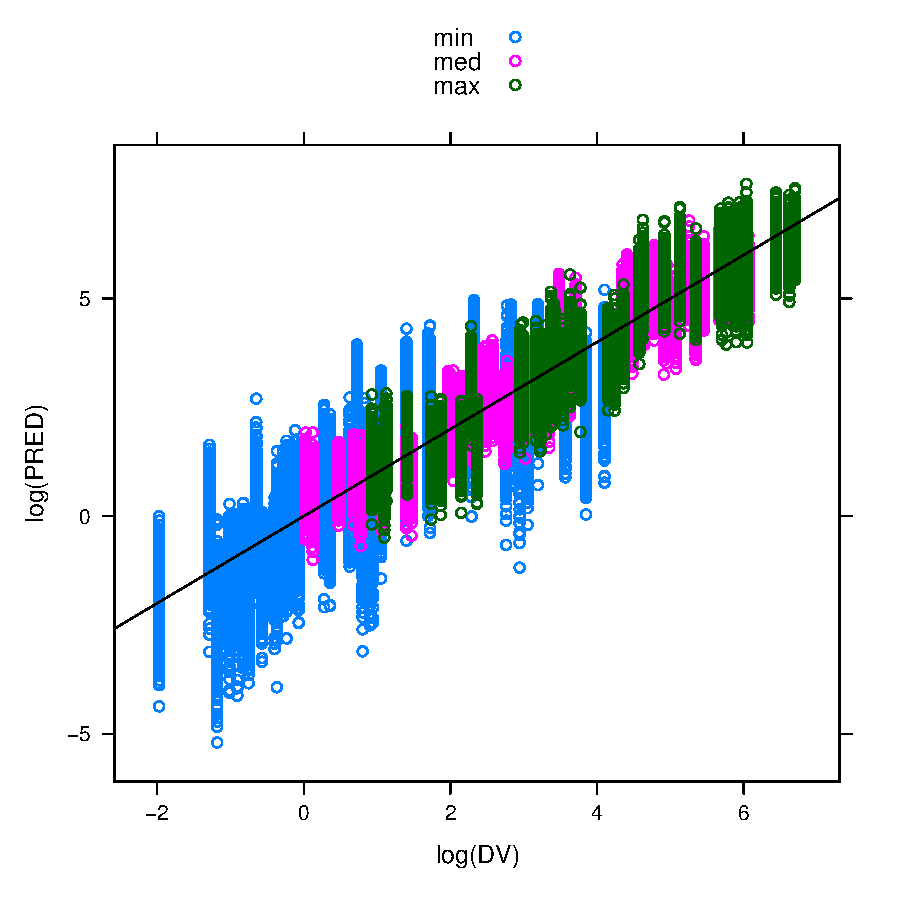
\includegraphics{model1-groupLogLog}
\subsubsection{Aggregate data across subjects, within simulations.}
Our predictions have central tendencies, which can vary by SIM.
Thus, our metrics as well have central tendencies that vary by SIM.
We want to represent the variability across SIMS by aggregating within SIM.
That means aggregating across subjects, within SIMS.  
There are many aggregation strategies, but we choose quantiles for a non-parametric 
result. Quantiles that 'clip' the tails of the distribution offer robustness against
number of SIMS (i.e., results less dependent on number of sims).  
Within each SIM, let's find for each metric the 5th, 50th, and 95th percentile.
We also want to do this for the original data set (requires some minor rearrangement).
\begin{Schunk}
\begin{Sinput}
> head(dvpred)
\end{Sinput}
\begin{Soutput}
  SUBJ SIM metric    DV     PRED
1    1   1    min 0.363 0.179320
2    1   1    med 1.610 1.965300
3    1   1    max 3.090 5.031400
4    1   2    min 0.363 0.096462
5    1   2    med 1.610 3.044800
6    1   2    max 3.090 7.472800
\end{Soutput}
\begin{Sinput}
> quants <- melt(dvpred,measure.var=c('DV','PRED'))
> head(quants)
\end{Sinput}
\begin{Soutput}
  SUBJ SIM metric variable value
1    1   1    min       DV 0.363
2    1   1    med       DV 1.610
3    1   1    max       DV 3.090
4    1   2    min       DV 0.363
5    1   2    med       DV 1.610
6    1   2    max       DV 3.090
\end{Soutput}
\begin{Sinput}
> quants <- data.frame(cast(quants,SIM + metric + variable ~ .,fun=quantile,probs=c(0.05,0.50,0.95)))
> head(quants,10)
\end{Sinput}
\begin{Soutput}
   SIM metric variable       X5.    X50.     X95.
1    1    min       DV 0.3054500  2.1450  36.0750
2    1    min     PRED 0.0976828  2.3129  29.6127
3    1    med       DV 1.5860000 20.2500 290.2000
4    1    med     PRED 2.2552400 22.8675 304.0180
5    1    max       DV 3.0855000 40.7000 634.2500
6    1    max     PRED 4.4729900 47.2865 579.6585
7    2    min       DV 0.3054500  2.1450  36.0750
8    2    min     PRED 0.0949232  2.8080  32.3266
9    2    med       DV 1.5860000 20.2500 290.2000
10   2    med     PRED 1.6609825 23.4225 263.8535
\end{Soutput}
\end{Schunk}
Note, again, that DV quantiles are invariant across SIMS.
\subsubsection{Reformat data for bivariate display.}
We now have a lot of display options.  The simplest is to plot DV~PRED for each quantile and metric.
Requires slight rearrangement.
\begin{Schunk}
\begin{Sinput}
> molten <- melt(quants, measure.var=c('X5.','X50.','X95.'),variable_name='quant')
> head(molten)
\end{Sinput}
\begin{Soutput}
  SIM metric variable quant     value
1   1    min       DV   X5. 0.3054500
2   1    min     PRED   X5. 0.0976828
3   1    med       DV   X5. 1.5860000
4   1    med     PRED   X5. 2.2552400
5   1    max       DV   X5. 3.0855000
6   1    max     PRED   X5. 4.4729900
\end{Soutput}
\begin{Sinput}
> frozen <- data.frame(cast(molten, SIM + metric + quant ~ variable))
> head(frozen)
\end{Sinput}
\begin{Soutput}
  SIM metric quant        DV        PRED
1   1    min   X5.   0.30545   0.0976828
2   1    min  X50.   2.14500   2.3129000
3   1    min  X95.  36.07500  29.6127000
4   1    med   X5.   1.58600   2.2552400
5   1    med  X50.  20.25000  22.8675000
6   1    med  X95. 290.20000 304.0180000
\end{Soutput}
\end{Schunk}
\subsubsection{Bivariate display of within-simulation aggregate metrics.}
\begin{Schunk}
\begin{Sinput}
> print(xyplot(
+ 	log(PRED)~log(DV)|metric,
+ 	frozen,
+ 	groups=quant,
+ 	layout=c(1,3),
+ 	auto.key=TRUE,
+ 	panel=function(...){
+ 		panel.xyplot(...)
+ 		panel.abline(a=0,b=1)
+ 	}
+ ))
\end{Sinput}
\end{Schunk}
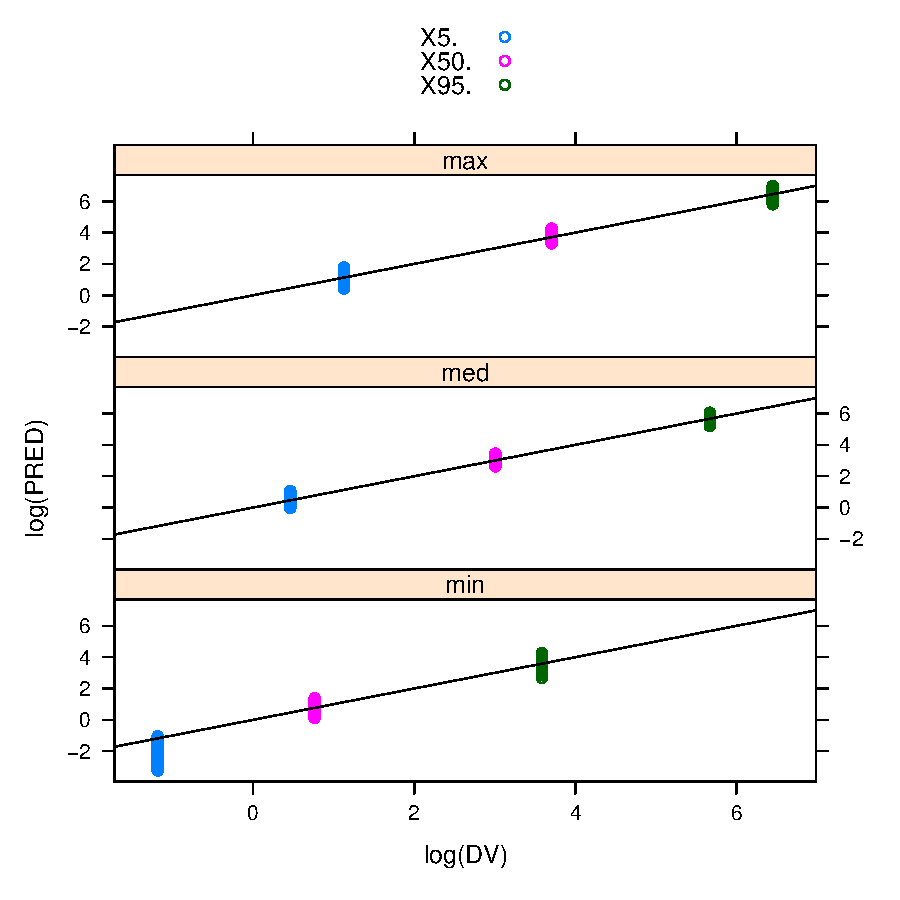
\includegraphics{model1-bivariate}
\subsubsection{Univariate displays.}
For a better view of the distributions, however, we can work with single-axis plot functions,
using the molten data.  For faster and clearer plotting, we remove duplicates of DV.
\subsubsection{Classic stripplot}
\begin{Schunk}
\begin{Sinput}
> head(molten)
\end{Sinput}
\begin{Soutput}
  SIM metric variable quant     value
1   1    min       DV   X5. 0.3054500
2   1    min     PRED   X5. 0.0976828
3   1    med       DV   X5. 1.5860000
4   1    med     PRED   X5. 2.2552400
5   1    max       DV   X5. 3.0855000
6   1    max     PRED   X5. 4.4729900
\end{Soutput}
\begin{Sinput}
> molten$SIM <- NULL
> table(molten$variable)
\end{Sinput}
\begin{Soutput}
  DV PRED 
4500 4500 
\end{Soutput}
\begin{Sinput}
> molten <- molten[!(duplicated(molten[,c('metric','variable','quant')]) & molten$variable=='DV'),]
> table(molten$variable)
\end{Sinput}
\begin{Soutput}
  DV PRED 
   9 4500 
\end{Soutput}
\begin{Sinput}
> library(grid)
> print(stripplot(
+ 	~value|metric+quant,
+ 	molten,
+ 	groups=variable,
+ 	horizontal=TRUE,
+ 	auto.key=TRUE,
+ 	panel=panel.superpose,
+ 	alpha=0.5,
+ 	panel.groups=panel.stripplot
+ ))
\end{Sinput}
\end{Schunk}
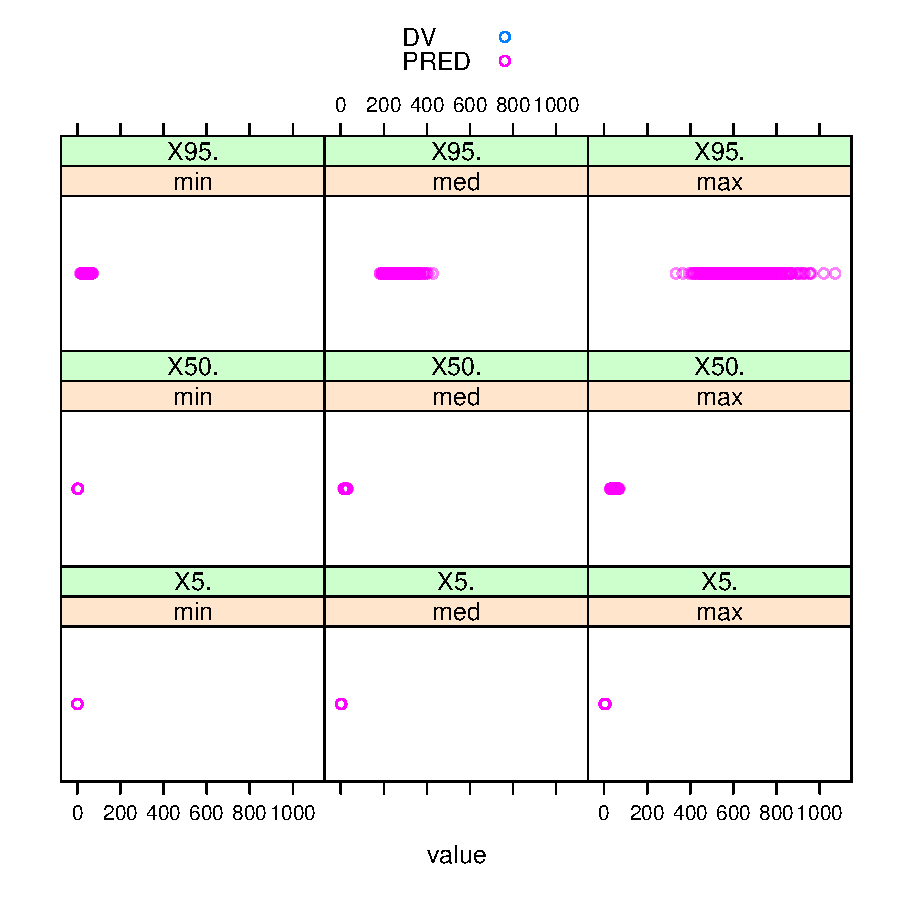
\includegraphics{model1-stripplot}
\subsubsection{Needle-in-the-haystack}
\begin{Schunk}
\begin{Sinput}
> print(stripplot(
+ 	~value|metric+quant,
+ 	molten,
+ 	groups=variable,
+ 	horizontal=TRUE,
+ 	auto.key=TRUE,
+ 	panel=panel.superpose,
+ 	alpha=0.5,
+ 	panel.groups=function(x,type,group.number,col.line,fill,col,...){
+ 		#browser()
+ 		view <- viewport(xscale=current.viewport()$xscale,yscale=c(0,max(hist(x,plot=FALSE)$density)))
+ 		pushViewport(view)
+ 		if(group.number==1) panel.abline(v=x,col=col.line)
+ 		else panel.histogram(x,breaks=NULL,col=fill,border=col.line,...)
+ 		popViewport()
+ 	}
+ ))
\end{Sinput}
\end{Schunk}
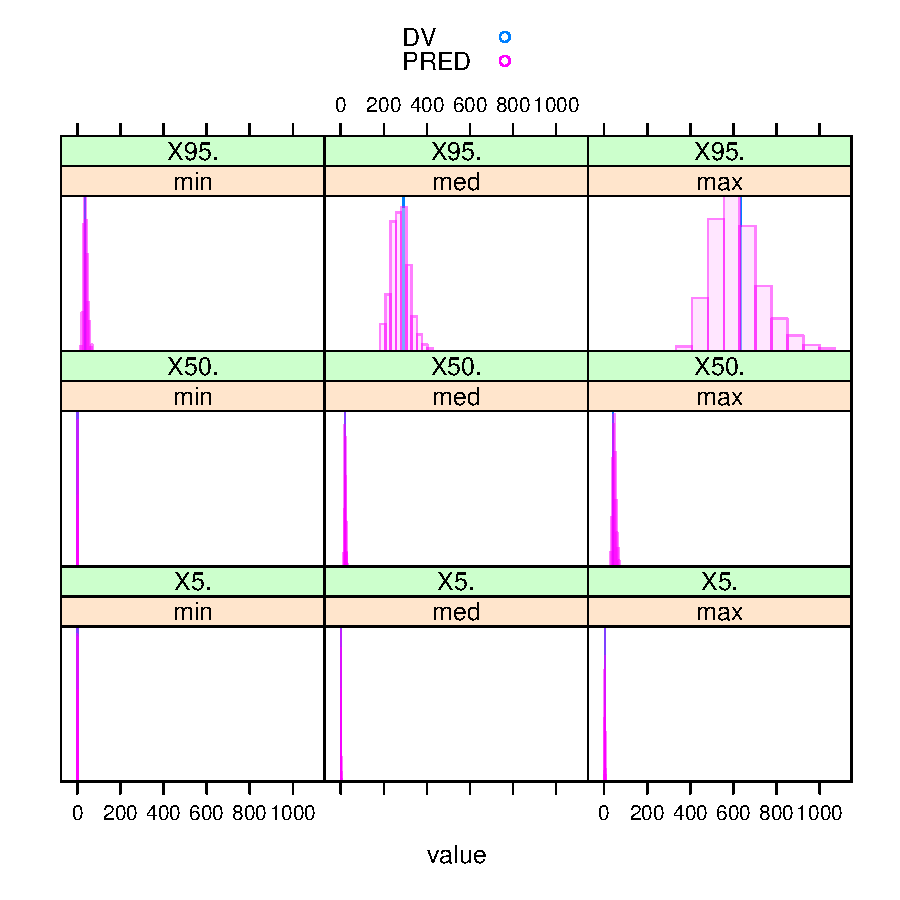
\includegraphics{model1-haystack}
\subsubsection{Haystacks in strips}
\begin{Schunk}
\begin{Sinput}
> print(stripplot(
+ 	quant~value|metric,
+ 	molten,
+ 	groups=variable,
+ 	auto.key=TRUE,
+ 	layout=c(1,3),
+ 	panel=panel.stratify,
+ 	alpha=0.5,
+ 	panel.levels=function(group.number,...){
+ 		if(group.number==1)panel.bar(...)
+ 		else panel.hist(...)
+ 	}
+ ))
\end{Sinput}
\end{Schunk}
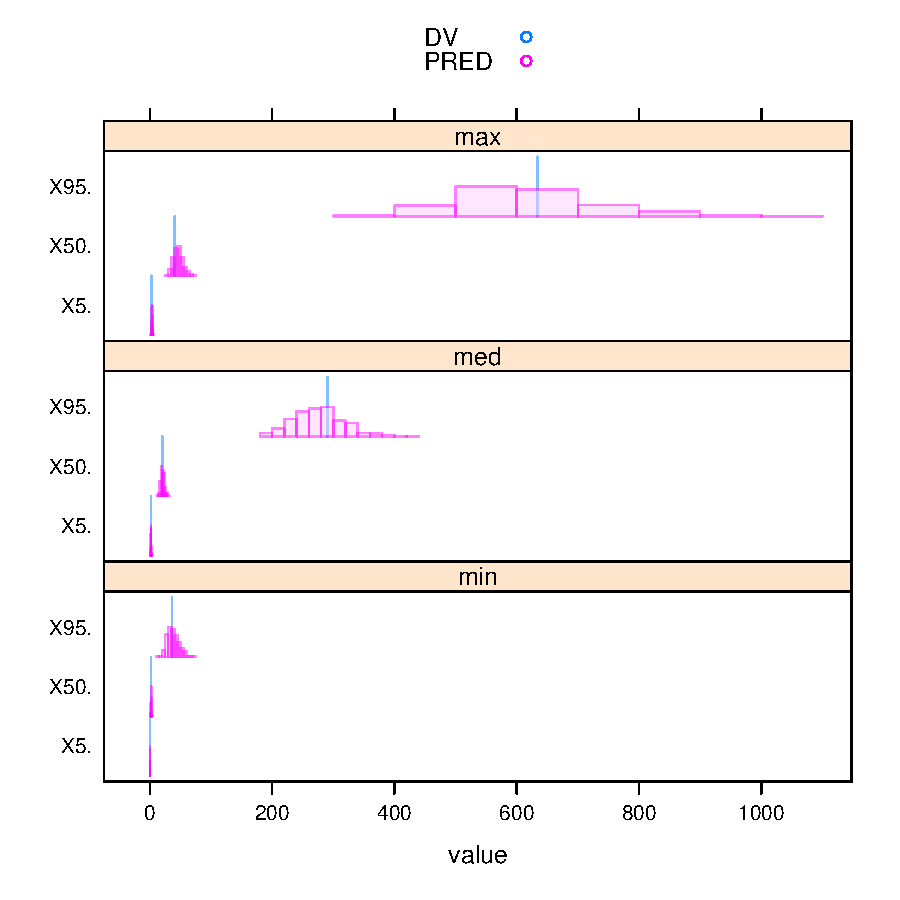
\includegraphics{model1-strippedHaystack}
\subsubsection{Density stripplot}
\begin{Schunk}
\begin{Sinput}
> print(stripplot(
+ 	~value|metric+quant,
+ 	molten,
+ 	groups=variable,
+ 	auto.key=TRUE,
+ 	panel=panel.stratify,
+ 	alpha=0.5,
+ 	panel.levels = function(group.number,x,y,font,col,col.line,...){
+ 		if(group.number==1)panel.segments(x0=x,x1=x,y0=y,y1=y+1,col=col.line,...)
+ 		else panel.densitystrip(x=x,y=y,col.line=col.line,...)
+ 	}
+ ))
\end{Sinput}
\end{Schunk}
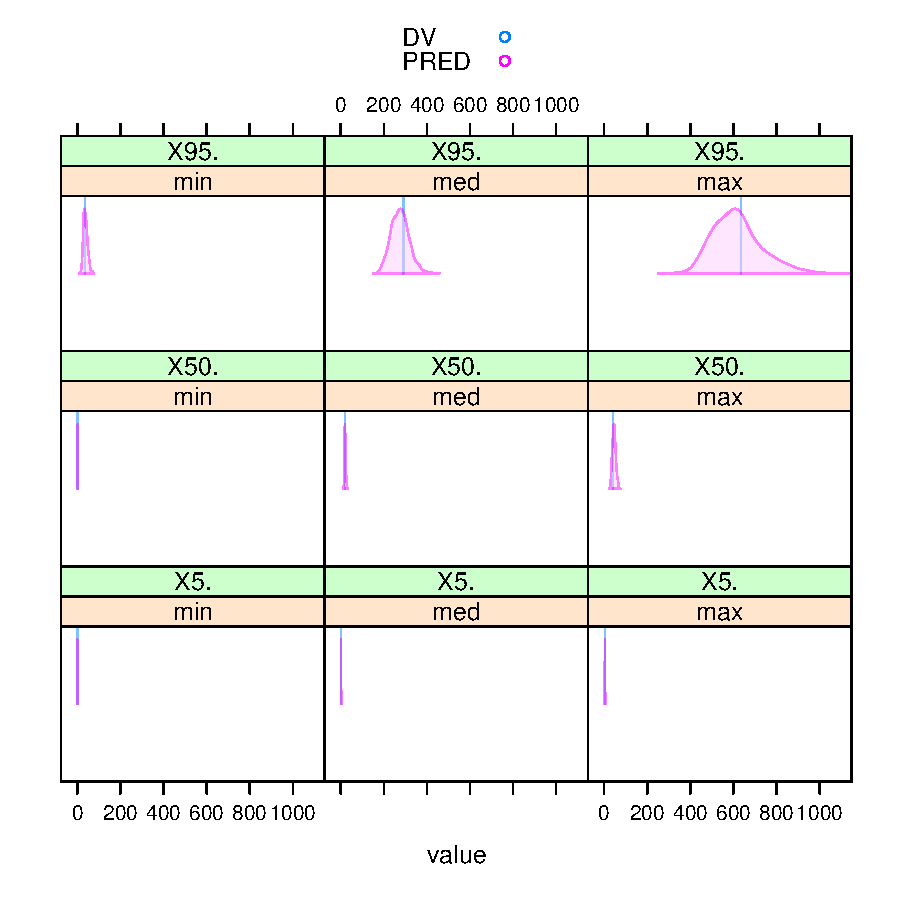
\includegraphics{model1-boa}
\subsubsection{Density variant: multistrip panels}
\begin{Schunk}
\begin{Sinput}
> print(stripplot(
+ 	quant~value|metric,
+ 	molten,
+ 	groups=variable,
+ 	auto.key=TRUE,
+ 	panel=panel.stratify,
+ 	alpha=0.5,
+ 	layout=c(1,3),
+ 	#scales=list(relation='free'),
+ 	panel.levels = function(x,y,group.number,col,col.line,fill,font,...){
+ 		if(group.number==1)panel.segments(x0=x,x1=x,y0=y,y1=y+1,col=col.line,...)
+ 		else panel.densitystrip(x=x,y=y,col=fill,border=col.line,...)
+ 	}
+ ))
\end{Sinput}
\end{Schunk}
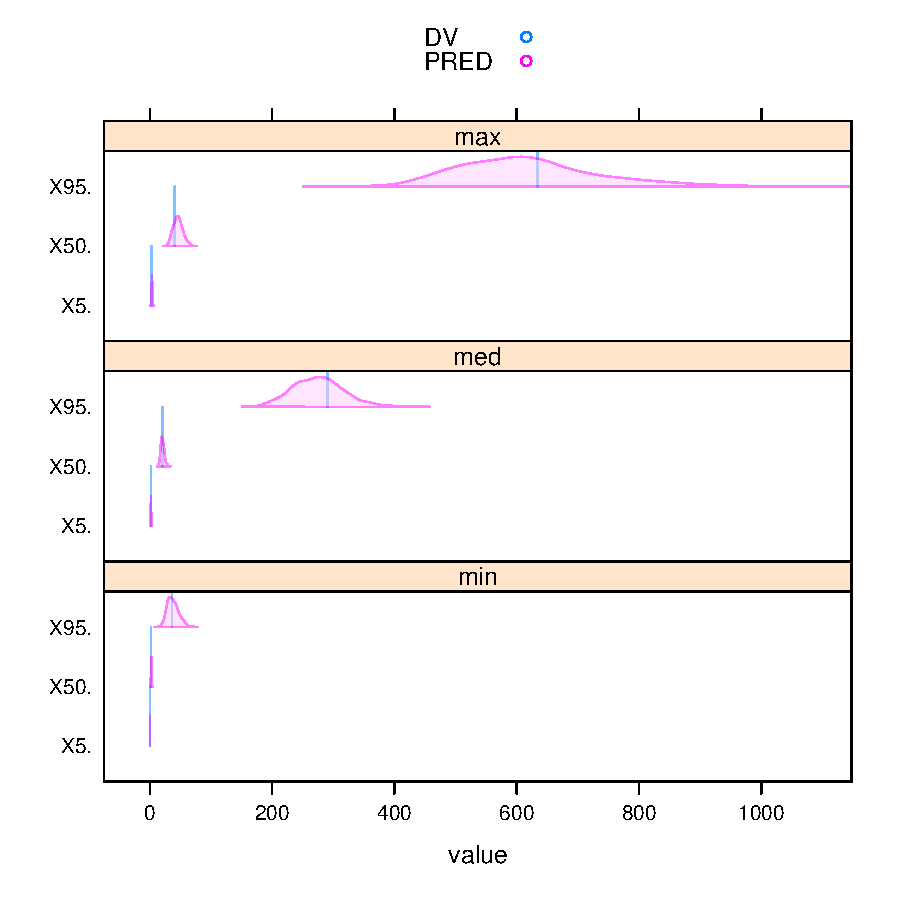
\includegraphics{model1-boa2}
\subsubsection{Density variant: interchanging the ordinal and the conditional}
\begin{Schunk}
\begin{Sinput}
> print(stripplot(
+ 	metric~value|quant,
+ 	molten,
+ 	groups=variable,
+ 	horizontal=TRUE,
+ 	auto.key=TRUE,
+ 	panel=panel.stratify,
+ 	alpha=0.5,
+ 	layout=c(1,3),
+ 	scales=list(relation='free'),
+ 	panel.levels = function(x,y,group.number,col,col.line,fill,font,...){
+ 		if(group.number==1)panel.segments(x0=x,x1=x,y0=y,y1=y+0.5,col=col.line,...)
+ 		else panel.densitystrip(x=x,y=y,col=fill,border=col.line,...)
+ 	}
+ ))
\end{Sinput}
\end{Schunk}
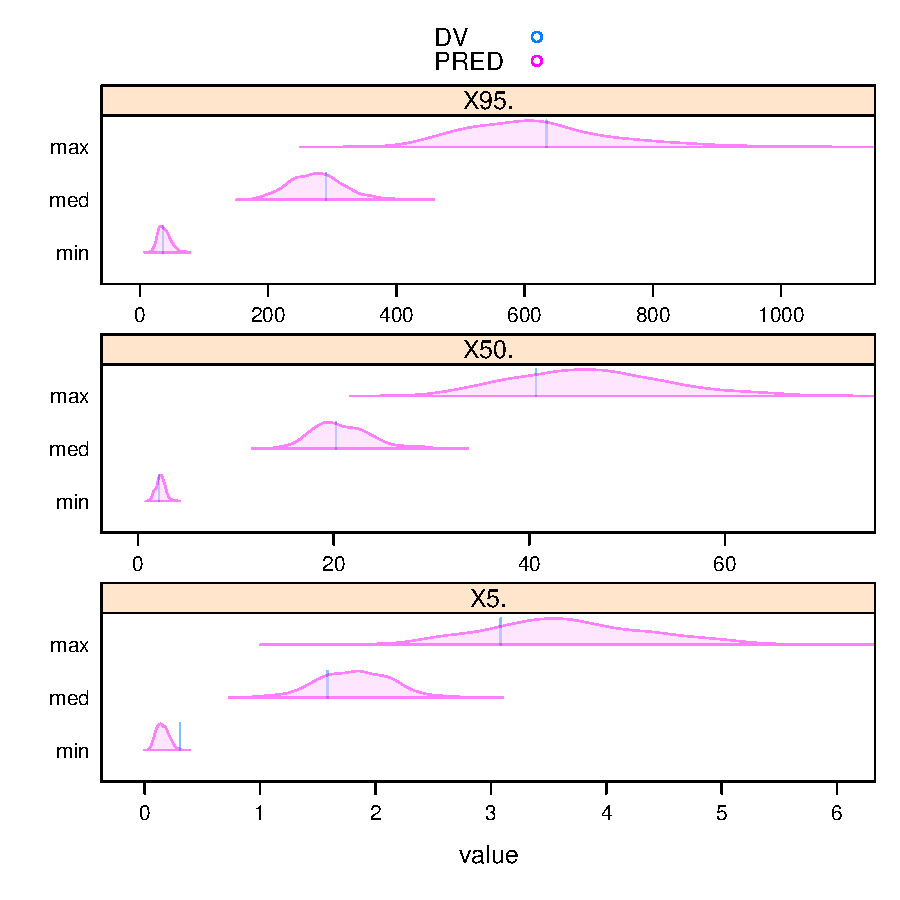
\includegraphics{model1-boa3}
\subsubsection{Diamondback: indicating reference regions}
It is often useful to show some reference region around a reference point estimate.
Here is one option.  
\begin{Schunk}
\begin{Sinput}
> print(stripplot(
+ 	metric~value|quant,
+ 	molten,
+ 	groups=variable,
+ 	auto.key=TRUE,
+ 	panel=panel.stratify,
+ 	alpha=0.5,
+ 	layout=c(1,3),
+ 	scales=list(relation='free'),
+ 	panel.levels = function(x,y,group.number,col,col.line,fill,font,...){
+ 		if(group.number==1)for(d in seq(length.out=length(x))) panel.polygon(
+ 			x=x[[d]]*c(0.8,1,1.25,1),
+ 			y=y[[d]] + c(0.25,0,0.25,0.5),
+ 			border=col.line,
+ 			col=fill,
+ 			...
+ 		)
+ 		else panel.densitystrip(x=x,y=y,col=fill,border=col.line,...)
+ 	}
+ ))
\end{Sinput}
\end{Schunk}
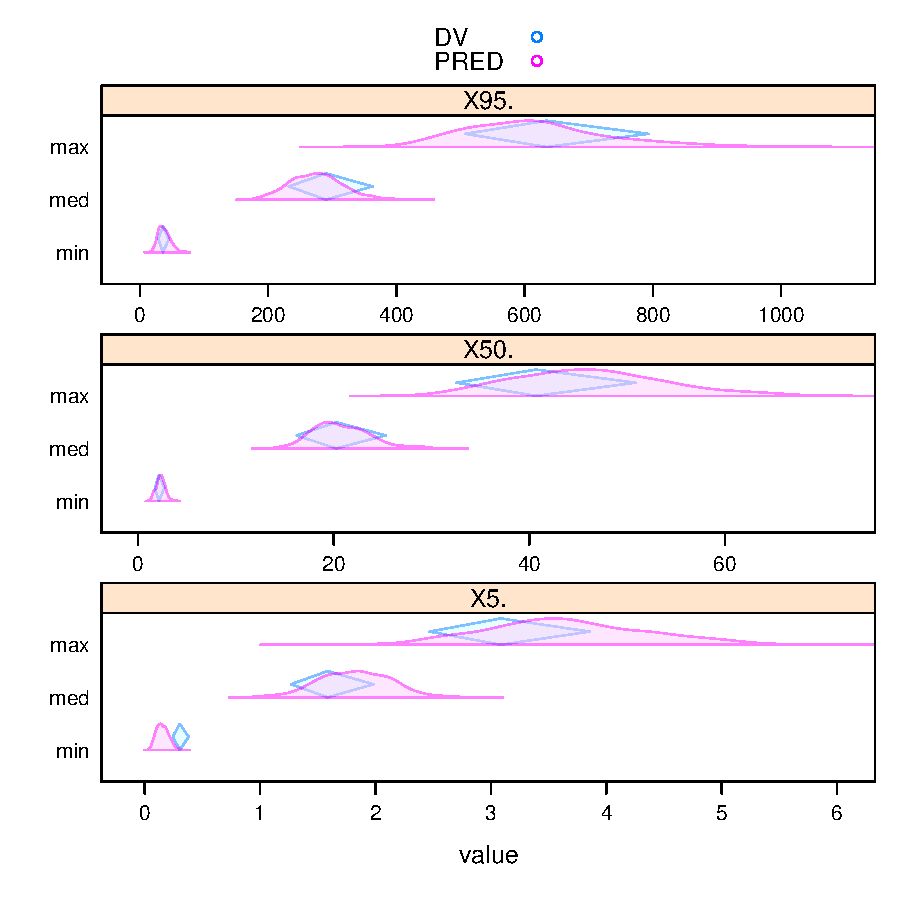
\includegraphics{model1-diamondBack}
\section{Bootstrap Estimates of Parameter Uncertainty}
\subsection{Create directories.}
\begin{Schunk}
\begin{Sinput}
> getwd()
\end{Sinput}
\begin{Soutput}
[1] "/Users/timb/project/metrum-mifuns/inst/mi210/script"
\end{Soutput}
\begin{Sinput}
> dir.create('../nonmem/1005.boot')
> dir.create('../nonmem/1005.boot/data')
> dir.create('../nonmem/1005.boot/ctl')
\end{Sinput}
\end{Schunk}
\subsection{Create replicate control streams.}
\begin{Schunk}
\begin{Sinput}
> t <- metaSub(
+      as.filename('../nonmem/ctl/1005.ctl'),
+      names=1:300,
+      pattern=c(
+          '1005',
+          '../../data/ph1/derived/phase1.csv',
+          '$COV',
+          '$TABLE'
+      ),
+      replacement=c(
+          '*',
+          '../data/*.csv',
+          ';$COV',
+          ';$TABLE'
+     ),
+     fixed=TRUE,
+     out='../nonmem/1005.boot/ctl',
+     suffix='.ctl'
+  )
\end{Sinput}
\end{Schunk}
\subsection{Create replicate data sets by resampling original.}
\begin{Schunk}
\begin{Sinput}
>  bootset <- read.csv('../data/ph1/derived/phase1.csv')
>  r <- resample(
+  	bootset,
+  	names=1:300,
+  	key='ID',
+  	rekey=TRUE,
+  	out='../nonmem/1005.boot/data',
+  	stratify='SEX'
+  )
\end{Sinput}
\end{Schunk}
\subsection{Run bootstrap models.}
Again, model step is commented for safety.  Run manually.
\begin{Schunk}
\begin{Sinput}
> #NONR(
> #     run=1:300,
> #     command=command,
> #     project='../nonmem/1005.boot/',
> #     boot=TRUE,
> #     nice=TRUE,
> #     streams='../nonmem/1005.boot/ctl'
> #)
> getwd()  
\end{Sinput}
\begin{Soutput}
[1] "/Users/timb/project/metrum-mifuns/inst/mi210/script"
\end{Soutput}
\end{Schunk}
\subsection{Summarize bootstrap models.}
When the bootstraps are complete, we return here and summarize. If you 
do not have time for bootstraps, use read.csv() on ../nonmem/1005.boot/log.csv.
\begin{Schunk}
\begin{Sinput}
> #boot <- read.csv('../nonmem/1005.boot/log.csv',as.is=TRUE) 
> boot <- rlog(
+ 	run=1:300,
+ 	project='../nonmem/1005.boot',
+ 	boot=TRUE,
+ 	append=FALSE,
+ 	tool='nm7'
+ )
> head(boot)
\end{Sinput}
\begin{Soutput}
  tool run parameter   moment                                            value
1  nm7   1      prob     text 1 phase1 2 CMT like 1004 but diff. initial on V3
2  nm7   1       min   status                                                0
3  nm7   1       ofv estimate                                 2760.84241850239
4  nm7   1  OMEGA1.1 estimate                                         0.188595
5  nm7   1  OMEGA1.1     prse                                             <NA>
6  nm7   1  OMEGA2.1 estimate                                                0
\end{Soutput}
\begin{Sinput}
> unique(boot$parameter)
\end{Sinput}
\begin{Soutput}
 [1] "prob"     "min"      "ofv"      "OMEGA1.1" "OMEGA2.1" "OMEGA2.2"
 [7] "OMEGA3.1" "OMEGA3.2" "OMEGA3.3" "SIGMA1.1" "THETA1"   "THETA2"  
[13] "THETA3"   "THETA4"   "THETA5"   "THETA6"   "THETA7"  
\end{Soutput}
\begin{Sinput}
> text2decimal(unique(boot$parameter))
\end{Sinput}
\begin{Soutput}
 [1]  NA  NA  NA 1.1 2.1 2.2 3.1 3.2 3.3 1.1 1.0 2.0 3.0 4.0 5.0 6.0 7.0
\end{Soutput}
\end{Schunk}
It looks like we have 14 estimated parameters.  We will map them to the
original control stream.
\begin{Schunk}
\begin{Sinput}
> boot <- boot[!is.na(text2decimal(boot$parameter)),]
> head(boot)
\end{Sinput}
\begin{Soutput}
  tool run parameter   moment    value
4  nm7   1  OMEGA1.1 estimate 0.188595
5  nm7   1  OMEGA1.1     prse     <NA>
6  nm7   1  OMEGA2.1 estimate        0
7  nm7   1  OMEGA2.1     prse     <NA>
8  nm7   1  OMEGA2.2 estimate 0.112992
9  nm7   1  OMEGA2.2     prse     <NA>
\end{Soutput}
\begin{Sinput}
> unique(boot$moment)
\end{Sinput}
\begin{Soutput}
[1] "estimate" "prse"    
\end{Soutput}
\begin{Sinput}
> unique(boot$value[boot$moment=='prse'])
\end{Sinput}
\begin{Soutput}
[1] NA
\end{Soutput}
\end{Schunk}
prse, and therefore moment, is noninformative for these bootstraps.
\begin{Schunk}
\begin{Sinput}
> boot <- boot[boot$moment=='estimate',]
> boot$moment <- NULL
> unique(boot$tool)
\end{Sinput}
\begin{Soutput}
[1] "nm7"
\end{Soutput}
\begin{Sinput}
> boot$tool <- NULL
> head(boot)
\end{Sinput}
\begin{Soutput}
   run parameter     value
4    1  OMEGA1.1  0.188595
6    1  OMEGA2.1         0
8    1  OMEGA2.2  0.112992
10   1  OMEGA3.1         0
12   1  OMEGA3.2         0
14   1  OMEGA3.3 0.0854714
\end{Soutput}
\begin{Sinput}
> unique(boot$value[boot$parameter %in% c('OMEGA2.1','OMEGA3.1','OMEGA3.2')])
\end{Sinput}
\begin{Soutput}
[1] "0"
\end{Soutput}
\begin{Sinput}
> unique(boot$parameter[boot$value=='0'])
\end{Sinput}
\begin{Soutput}
[1] "OMEGA2.1" "OMEGA3.1" "OMEGA3.2"
\end{Soutput}
\end{Schunk}
Off-diagonals (and only off-diagonals) are noninformative.
\begin{Schunk}
\begin{Sinput}
> boot <- boot[!boot$value=='0',]
> any(is.na(as.numeric(boot$value)))
\end{Sinput}
\begin{Soutput}
[1] FALSE
\end{Soutput}
\begin{Sinput}
> boot$value <- as.numeric(boot$value)
> head(boot)
\end{Sinput}
\begin{Soutput}
   run parameter      value
4    1  OMEGA1.1  0.1885950
8    1  OMEGA2.2  0.1129920
14   1  OMEGA3.3  0.0854714
16   1  SIGMA1.1  0.0640717
18   1    THETA1  7.9889300
20   1    THETA2 19.8920000
\end{Soutput}
\end{Schunk}
\subsection{Restrict data to 95 percentiles.}
We did 300 runs.  Min and max are strongly dependent on number of runs, since 
with an unbounded distribution, (almost) any value is possible with enough sampling.
We clip to the 95 percentiles, to give distributions that are somewhat more
scale independent.
\begin{Schunk}
\begin{Sinput}
> boot$upper <- with(boot,reapply(value,INDEX=parameter,FUN=quantile,probs=0.975))
> boot$lower <- with(boot,reapply(value,INDEX=parameter,FUN=quantile,probs=0.025))
> nrow(boot)
\end{Sinput}
\begin{Soutput}
[1] 3300
\end{Soutput}
\begin{Sinput}
> boot <- boot[with(boot, value < upper & value > lower),]
> nrow(boot)
\end{Sinput}
\begin{Soutput}
[1] 3124
\end{Soutput}
\begin{Sinput}
> head(boot)
\end{Sinput}
\begin{Soutput}
   run parameter      value       upper       lower
4    1  OMEGA1.1  0.1885950  0.28599012  0.10657525
8    1  OMEGA2.2  0.1129920  0.19930930  0.05290951
14   1  OMEGA3.3  0.0854714  0.16658800  0.05277859
16   1  SIGMA1.1  0.0640717  0.08328707  0.05422743
18   1    THETA1  7.9889300 10.18006750  6.90182250
20   1    THETA2 19.8920000 26.29300250 17.74395750
\end{Soutput}
\begin{Sinput}
> boot$upper <- NULL
> boot$lower <- NULL
> head(boot)
\end{Sinput}
\begin{Soutput}
   run parameter      value
4    1  OMEGA1.1  0.1885950
8    1  OMEGA2.2  0.1129920
14   1  OMEGA3.3  0.0854714
16   1  SIGMA1.1  0.0640717
18   1    THETA1  7.9889300
20   1    THETA2 19.8920000
\end{Soutput}
\end{Schunk}
\subsection{Recover parameter metadata from a specially-marked control stream.}
We want meaningful names for our parameters.  Harvest these from a reviewed control
stream.
\begin{Schunk}
\begin{Sinput}
> stream <- readLines('../nonmem/ctl/1005.ctl')
> tail(stream)
\end{Sinput}
\begin{Soutput}
[1] "$SIGMA 0.09 ;0.1"                                                                
[2] ";<parameter name='SIGMA1.1' label='ERR'>proportional error</parameter>"          
[3] "$ESTIMATION MAXEVAL=9999 PRINT=5 NOABORT METHOD=1 INTER MSFO=./1005.msf"         
[4] "$COV PRINT=E"                                                                    
[5] "$TABLE NOPRINT FILE=./1005.tab ONEHEADER ID AMT TIME EVID PRED IPRE CWRES"       
[6] "$TABLE NOPRINT FILE=./1005par.tab ONEHEADER ID TIME CL Q V2 V3 KA ETA1 ETA2 ETA3"
\end{Soutput}
\begin{Sinput}
> doc <- ctl2xml(stream)
> doc
\end{Sinput}
\begin{Soutput}
 [1] "<document>"                                                                                         
 [2] "<parameter name='THETA1' label='CL'>clearance</parameter>"                                          
 [3] "<parameter name='THETA2' label='V2'>central volume</parameter>"                                     
 [4] "<parameter name='THETA3' label='Ka'>absorption constant</parameter>"                                
 [5] "<parameter name='THETA4' label='Q' >intercompartmental clearance</parameter>"                       
 [6] "<parameter name='THETA5' label='V3'>peripheral volume</parameter>"                                  
 [7] "<parameter name='THETA6' label='Male.CL'>male effect on clearance</parameter>"                      
 [8] "<parameter name='THETA7' label='WT.CL'>weight effect on clearance</parameter>"                      
 [9] "<parameter name='OMEGA1.1' label='IIV.CL'>interindividual variability on clearance</parameter>"     
[10] "<parameter name='OMEGA2.1' label='CL.V2'>covariance of clearance and central volume</parameter>"    
[11] "<parameter name='OMEGA2.2' label='IIV.V2'>interindividual variability on central volume</parameter>"
[12] "<parameter name='OMEGA3.1' label='CL.Ka'>covariance of clearance and Ka</parameter>"                
[13] "<parameter name='OMEGA3.2' label='V2.Ka'>covariance of central volume and Ka</parameter>"           
[14] "<parameter name='OMEGA3.3' label='IIV.Ka'>interindividual variability on Ka</parameter>"            
[15] "<parameter name='SIGMA1.1' label='ERR'>proportional error</parameter>"                              
[16] "</document>"                                                                                        
\end{Soutput}
\begin{Sinput}
> params <- unique(boot[,'parameter',drop=FALSE])
> params$defs <- lookup(params$parameter,within=doc)
> params$labels <- lookup(params$parameter,within=doc,as='label')
> params
\end{Sinput}
\begin{Soutput}
   parameter                                          defs  labels
4   OMEGA1.1      interindividual variability on clearance  IIV.CL
8   OMEGA2.2 interindividual variability on central volume  IIV.V2
14  OMEGA3.3             interindividual variability on Ka  IIV.Ka
16  SIGMA1.1                            proportional error     ERR
18    THETA1                                     clearance      CL
20    THETA2                                central volume      V2
22    THETA3                           absorption constant      Ka
24    THETA4                  intercompartmental clearance       Q
26    THETA5                             peripheral volume      V3
28    THETA6                      male effect on clearance Male.CL
30    THETA7                    weight effect on clearance   WT.CL
\end{Soutput}
\begin{Sinput}
> boot$parameter <- lookup(boot$parameter,within=doc,as='label')
> head(boot)
\end{Sinput}
\begin{Soutput}
   run parameter      value
4    1    IIV.CL  0.1885950
8    1    IIV.V2  0.1129920
14   1    IIV.Ka  0.0854714
16   1       ERR  0.0640717
18   1        CL  7.9889300
20   1        V2 19.8920000
\end{Soutput}
\end{Schunk}
\subsection{Create covariate plot.}
Now we make a covariate plot for clearance.  We will normalize clearance 
by its median (we also could have used the model estimate).  We need to take 
cuts of weight, since we can only really show categorically-constrained distributions.
Male effect is already categorical.  I.e, the reference individual has median
clearance, is female, and has median weight.
\subsubsection{Recover original covariates for guidance.}
\begin{Schunk}
\begin{Sinput}
> covariates <- read.csv('../data/ph1/derived/phase1.csv',na.strings='.')
> head(covariates)
\end{Sinput}
\begin{Soutput}
     C ID TIME SEQ EVID  AMT    DV SUBJ HOUR TAFD  TAD LDOS MDV HEIGHT WEIGHT
1    C  1 0.00   0    0   NA 0.000    1 0.00 0.00   NA   NA   0    174   74.2
2 <NA>  1 0.00   1    1 1000    NA    1 0.00 0.00 0.00 1000   1    174   74.2
3 <NA>  1 0.25   0    0   NA 0.363    1 0.25 0.25 0.25 1000   0    174   74.2
4 <NA>  1 0.50   0    0   NA 0.914    1 0.50 0.50 0.50 1000   0    174   74.2
5 <NA>  1 1.00   0    0   NA 1.120    1 1.00 1.00 1.00 1000   0    174   74.2
6 <NA>  1 2.00   0    0   NA 2.280    1 2.00 2.00 2.00 1000   0    174   74.2
  SEX  AGE DOSE FED SMK DS CRCN predose zerodv
1   0 29.1 1000   1   0  0 83.5       1      1
2   0 29.1 1000   1   0  0 83.5       0      0
3   0 29.1 1000   1   0  0 83.5       0      0
4   0 29.1 1000   1   0  0 83.5       0      0
5   0 29.1 1000   1   0  0 83.5       0      0
6   0 29.1 1000   1   0  0 83.5       0      0
\end{Soutput}
\begin{Sinput}
> with(covariates,constant(WEIGHT,within=ID))
\end{Sinput}
\begin{Soutput}
[1] TRUE
\end{Soutput}
\begin{Sinput}
> covariates <- unique(covariates[,c('ID','WEIGHT')])
> head(covariates)
\end{Sinput}
\begin{Soutput}
   ID WEIGHT
1   1   74.2
16  2   80.3
31  3   94.2
46  4   85.2
61  5   82.8
76  6   63.9
\end{Soutput}
\begin{Sinput}
> covariates$WT <- as.numeric(covariates$WEIGHT)
> wt <- median(covariates$WT)
> wt
\end{Sinput}
\begin{Soutput}
[1] 81
\end{Soutput}
\begin{Sinput}
> range(covariates$WT)
\end{Sinput}
\begin{Soutput}
[1]  61 117
\end{Soutput}
\end{Schunk}
\subsubsection{Reproduce the control stream submodel for selective cuts of a continuous covariate.}
In the model we normalized by 70 kg, so that cut will have null effect.
Let's try 65, 75, and 85 kg. We have to make a separate column for each
cut, which is a bit of work. Basically, we make two more copies of our
weight effect columns, and raise our normalized cuts to those powers, 
effectively reproducing the submodel from the control stream.
\begin{Schunk}
\begin{Sinput}
> head(boot) 
\end{Sinput}
\begin{Soutput}
   run parameter      value
4    1    IIV.CL  0.1885950
8    1    IIV.V2  0.1129920
14   1    IIV.Ka  0.0854714
16   1       ERR  0.0640717
18   1        CL  7.9889300
20   1        V2 19.8920000
\end{Soutput}
\begin{Sinput}
> clearance <- boot[boot$parameter %in% c('CL','WT.CL','Male.CL'),]
> head(clearance)
\end{Sinput}
\begin{Soutput}
   run parameter    value
18   1        CL 7.988930
28   1   Male.CL 1.182580
30   1     WT.CL 1.308790
49   2        CL 7.636730
59   2   Male.CL 0.956565
61   2     WT.CL 2.369810
\end{Soutput}
\begin{Sinput}
> frozen <- data.frame(cast(clearance,run~parameter))
> head(frozen)
\end{Sinput}
\begin{Soutput}
  run      CL  Male.CL   WT.CL
1   1 7.98893 1.182580 1.30879
2  10 9.85489 0.836765 1.85115
3 100 8.77202 0.916888 1.63059
4 101 7.52437 1.121880 1.58567
5 102 9.70459 1.003720 1.32105
6 103 9.57681 0.966337 1.69517
\end{Soutput}
\begin{Sinput}
> frozen$WT.CL65 <- (60/70)**frozen$WT.CL
> frozen$WT.CL75 <- (75/70)**frozen$WT.CL
> frozen$WT.CL85 <- (85/70)**frozen$WT.CL
\end{Sinput}
\end{Schunk}
\subsubsection{Normalize key parameter}
\begin{Schunk}
\begin{Sinput}
> cl <- median(boot$value[boot$parameter=='CL'])
> cl
\end{Sinput}
\begin{Soutput}
[1] 8.56139
\end{Soutput}
\begin{Sinput}
> frozen$CL <- frozen$CL/cl
> head(frozen)
\end{Sinput}
\begin{Soutput}
  run        CL  Male.CL   WT.CL   WT.CL65  WT.CL75  WT.CL85
1   1 0.9331347 1.182580 1.30879 0.8172985 1.094499 1.289313
2  10 1.1510853 0.836765 1.85115 0.7517466 1.136230 1.432487
3 100 1.0246023 0.916888 1.63059 0.7777450 1.119071 1.372438
4 101 0.8788725 1.121880 1.58567 0.7831492 1.115608 1.360521
5 102 1.1335297 1.003720 1.32105 0.8157554 1.095426 1.292386
6 103 1.1186046 0.966337 1.69517 0.7700409 1.124068 1.389755
\end{Soutput}
\begin{Sinput}
> frozen$WT.CL <- NULL
> molten <- melt(frozen,id.var='run',na.rm=TRUE)
> head(molten)
\end{Sinput}
\begin{Soutput}
  run variable     value
1   1       CL 0.9331347
2  10       CL 1.1510853
3 100       CL 1.0246023
4 101       CL 0.8788725
5 102       CL 1.1335297
6 103       CL 1.1186046
\end{Soutput}
\end{Schunk}
\subsubsection{Plot.}
Now we plot.  We reverse the variable factor to give us top-down layout
of strips.
\begin{Schunk}
\begin{Sinput}
> levels(molten$variable)
\end{Sinput}
\begin{Soutput}
[1] "CL"      "Male.CL" "WT.CL65" "WT.CL75" "WT.CL85"
\end{Soutput}
\begin{Sinput}
> print(stripplot(
+ 	factor(
+ 		variable,levels= c(
+ 			"WT.CL85",
+ 			"WT.CL75",
+ 			"WT.CL65",
+ 			"Male.CL",
+ 			"CL"
+ 		)
+ 	)~value,
+ 	molten,
+ 	panel=panel.covplot
+ ))
\end{Sinput}
\end{Schunk}
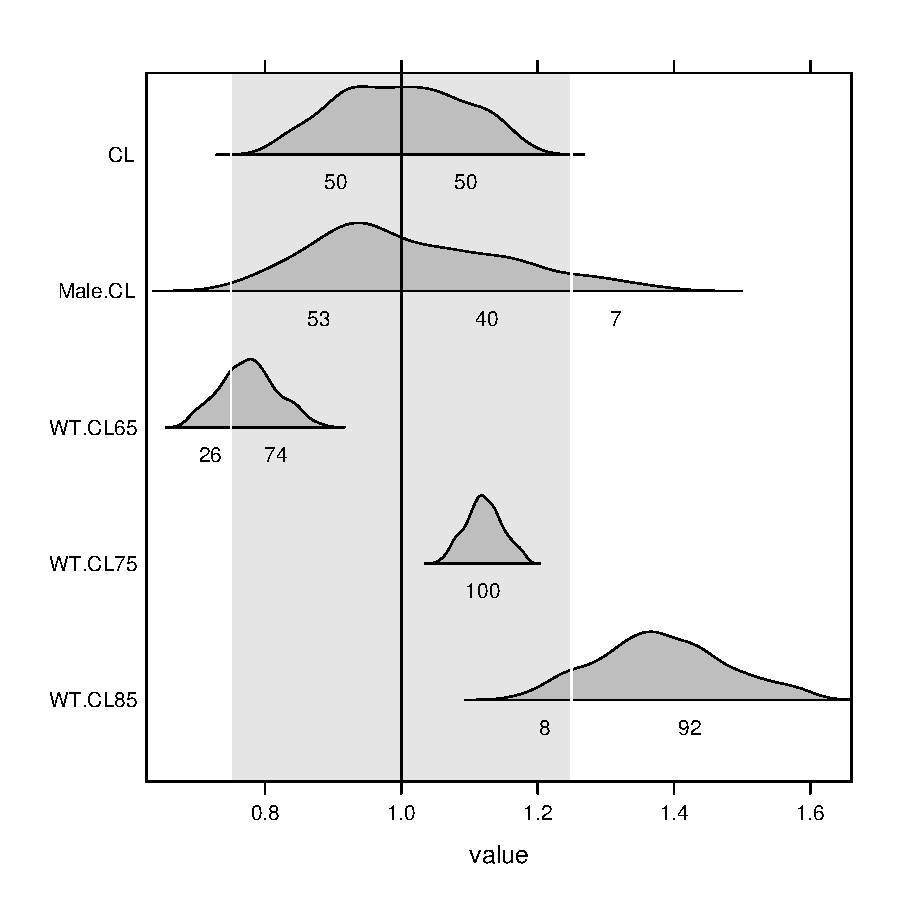
\includegraphics{model1-covplot}
Alternatively, we could use groups to collapse the continuous strips into a single band.
\begin{Schunk}
\begin{Sinput}
> levels(molten$variable)
\end{Sinput}
\begin{Soutput}
[1] "CL"      "Male.CL" "WT.CL65" "WT.CL75" "WT.CL85"
\end{Soutput}
\begin{Sinput}
> print(stripplot(
+ 	factor(factor(
+ 		variable,
+ 		levels= c(
+ 			"WT.CL85",
+ 			"WT.CL75",
+ 			"WT.CL65",
+ 			"Male.CL",
+ 			"CL"
+ 		),
+ 		labels=c(
+ 			'WT.CL',
+ 			'WT.CL',
+ 			'WT.CL',
+ 			'Male.CL',
+ 			'CL'
+ 		))
+ 	)~value,
+ 	molten,
+ 	groups=factor(
+ 		variable,
+ 		levels= c(
+ 			"WT.CL85",
+ 			"WT.CL75",
+ 			"WT.CL65",
+ 			"Male.CL",
+ 			"CL"
+ 		),
+ 		labels=c(
+ 			'85 kg',
+ 			'75 kg',
+ 			'65 kg',
+ 			'male',
+ 			'CL'
+ 		)
+ 	),
+ 	panel=panel.covplot,
+ 	auto.key=TRUE,
+ 	alpha=0.7
+ ))
\end{Sinput}
\end{Schunk}
\includegraphics{model1-groupcov}
\subsubsection{Summarize}
We see that clearance is estimated with good precision.  Ignoring outliers, there 
is not much effect on clearance of being male, relative to female.  Increasing 
weight is associated with increasing clearance.  There is a 79 percent probability
that an 85 kg person will have at least 25 percent greater clearance than a 70 kg
person.
\end{document}
















